\subsubsection{27.03.15 (Competition)}
\begin{center}
	1-st day of competition "FTC Dutch Open" in Eindhoven.
\end{center}

Today there was technical day. Also today we presented our engineering book to judges.\newline

As soon as we arrived at competition area, two of us started talking with other FTC teams. There were 48 teams on competition. We learned about opportunities and strategy of every team. We got data about all robots except two robots of teams from Saudi Arabia because their robots didn't arrived at Nederlands yet (they we transported as a luggage on another plane).\newline 
All the teams received from our team lists with short information about our strategy and opportunities. The background of our information list was the same to the background of the print on plexiglass protection of our robot which made our robot more noticable. So we did everything to attract others' teams attention and increase our chanses to be chosen by other teams for final matches.\newline
Between the teams we found two our friends (we kept in touch woth them since the central robofest in Moscow): team "Auto Vortex" from Romania and team "Trex" from Rissia.\newline

At the beginning of the day we presented engineering book. At first one of us told the judges about:
\begin{enumerate}
	\item Our team.
	
	\item Our strategy in game.
	
	\item Construction of the robot.
	
	\item Resourses we used in our work (LaTex, Creo Parametric 3.0, etc).
	
	\item Our coaches and sponsors.
	
\end{enumerate}
After that we all answered the judges' questions. After the presentation we realised, that our new way of telling it is more effective and we decided to follow this way in further presentations.\newline

When we were on hardware control, the judge criticized us for using for connecting the servos on the lift self-made wire. He permitted us to participate in this competition, but adviced us to change this wire to standard before the competition in USA because rules there are more strict.

Improvements that were done:
\begin{enumerate}
	\item For opening ball direct on the gutter during the game we linked it with the bucket by the thin wire instead of previous fishing line because it's easier to tie the wire than the line.
	\begin{figure}[H]
		\begin{minipage}[h]{0.2\linewidth}
			\center  
		\end{minipage}
		\begin{minipage}[h]{0.6\linewidth}
			\center{\includegraphics[scale=0.18]{days/27.03.15/images/01}}
			\caption{Stopper}
		\end{minipage}
	\end{figure}
	
	\item After a few trainings 2 servos on mechanism of overturning of the bucket broke down. The reason was that because of problems in mechanism of opening of the mechanism for directing balls vertically servos got extreme charge. Likely, we had an extra high-powered servo at the mechanism for capturing rolling goals. We installed this servo to the bucket overturner. 
	
	\item After that, we insalled two standard servomotors that we borrowed in teams "Trex" and "Auto Vortex" to the mechanism for capturing rolling goals.
	
	\item Then we solved the problem with opening the mechanism for directing balls vertically. Now the servo is able to overturn the bucket with five balls, but after we return to Russia we should install there the second one - in order to prolong servos' lifes.
	\begin{figure}[H]
		\begin{minipage}[h]{0.47\linewidth}
			\center{\includegraphics[scale=0.18]{days/27.03.15/images/01}}
			\caption{The cut corner}
		\end{minipage}
		\hfill
		\begin{minipage}[h]{0.47\linewidth}
			\center{\includegraphics[scale=0.2]{days/27.03.15/images/02}}
			\caption{Larger image}
		\end{minipage}
	\end{figure}
	
	\item We made special latches for the battery to prevent from falling out of the robot.
	\begin{figure}[H]
		\begin{minipage}[h]{0.2\linewidth}
			\center  
		\end{minipage}
		\begin{minipage}[h]{0.6\linewidth}
			\center{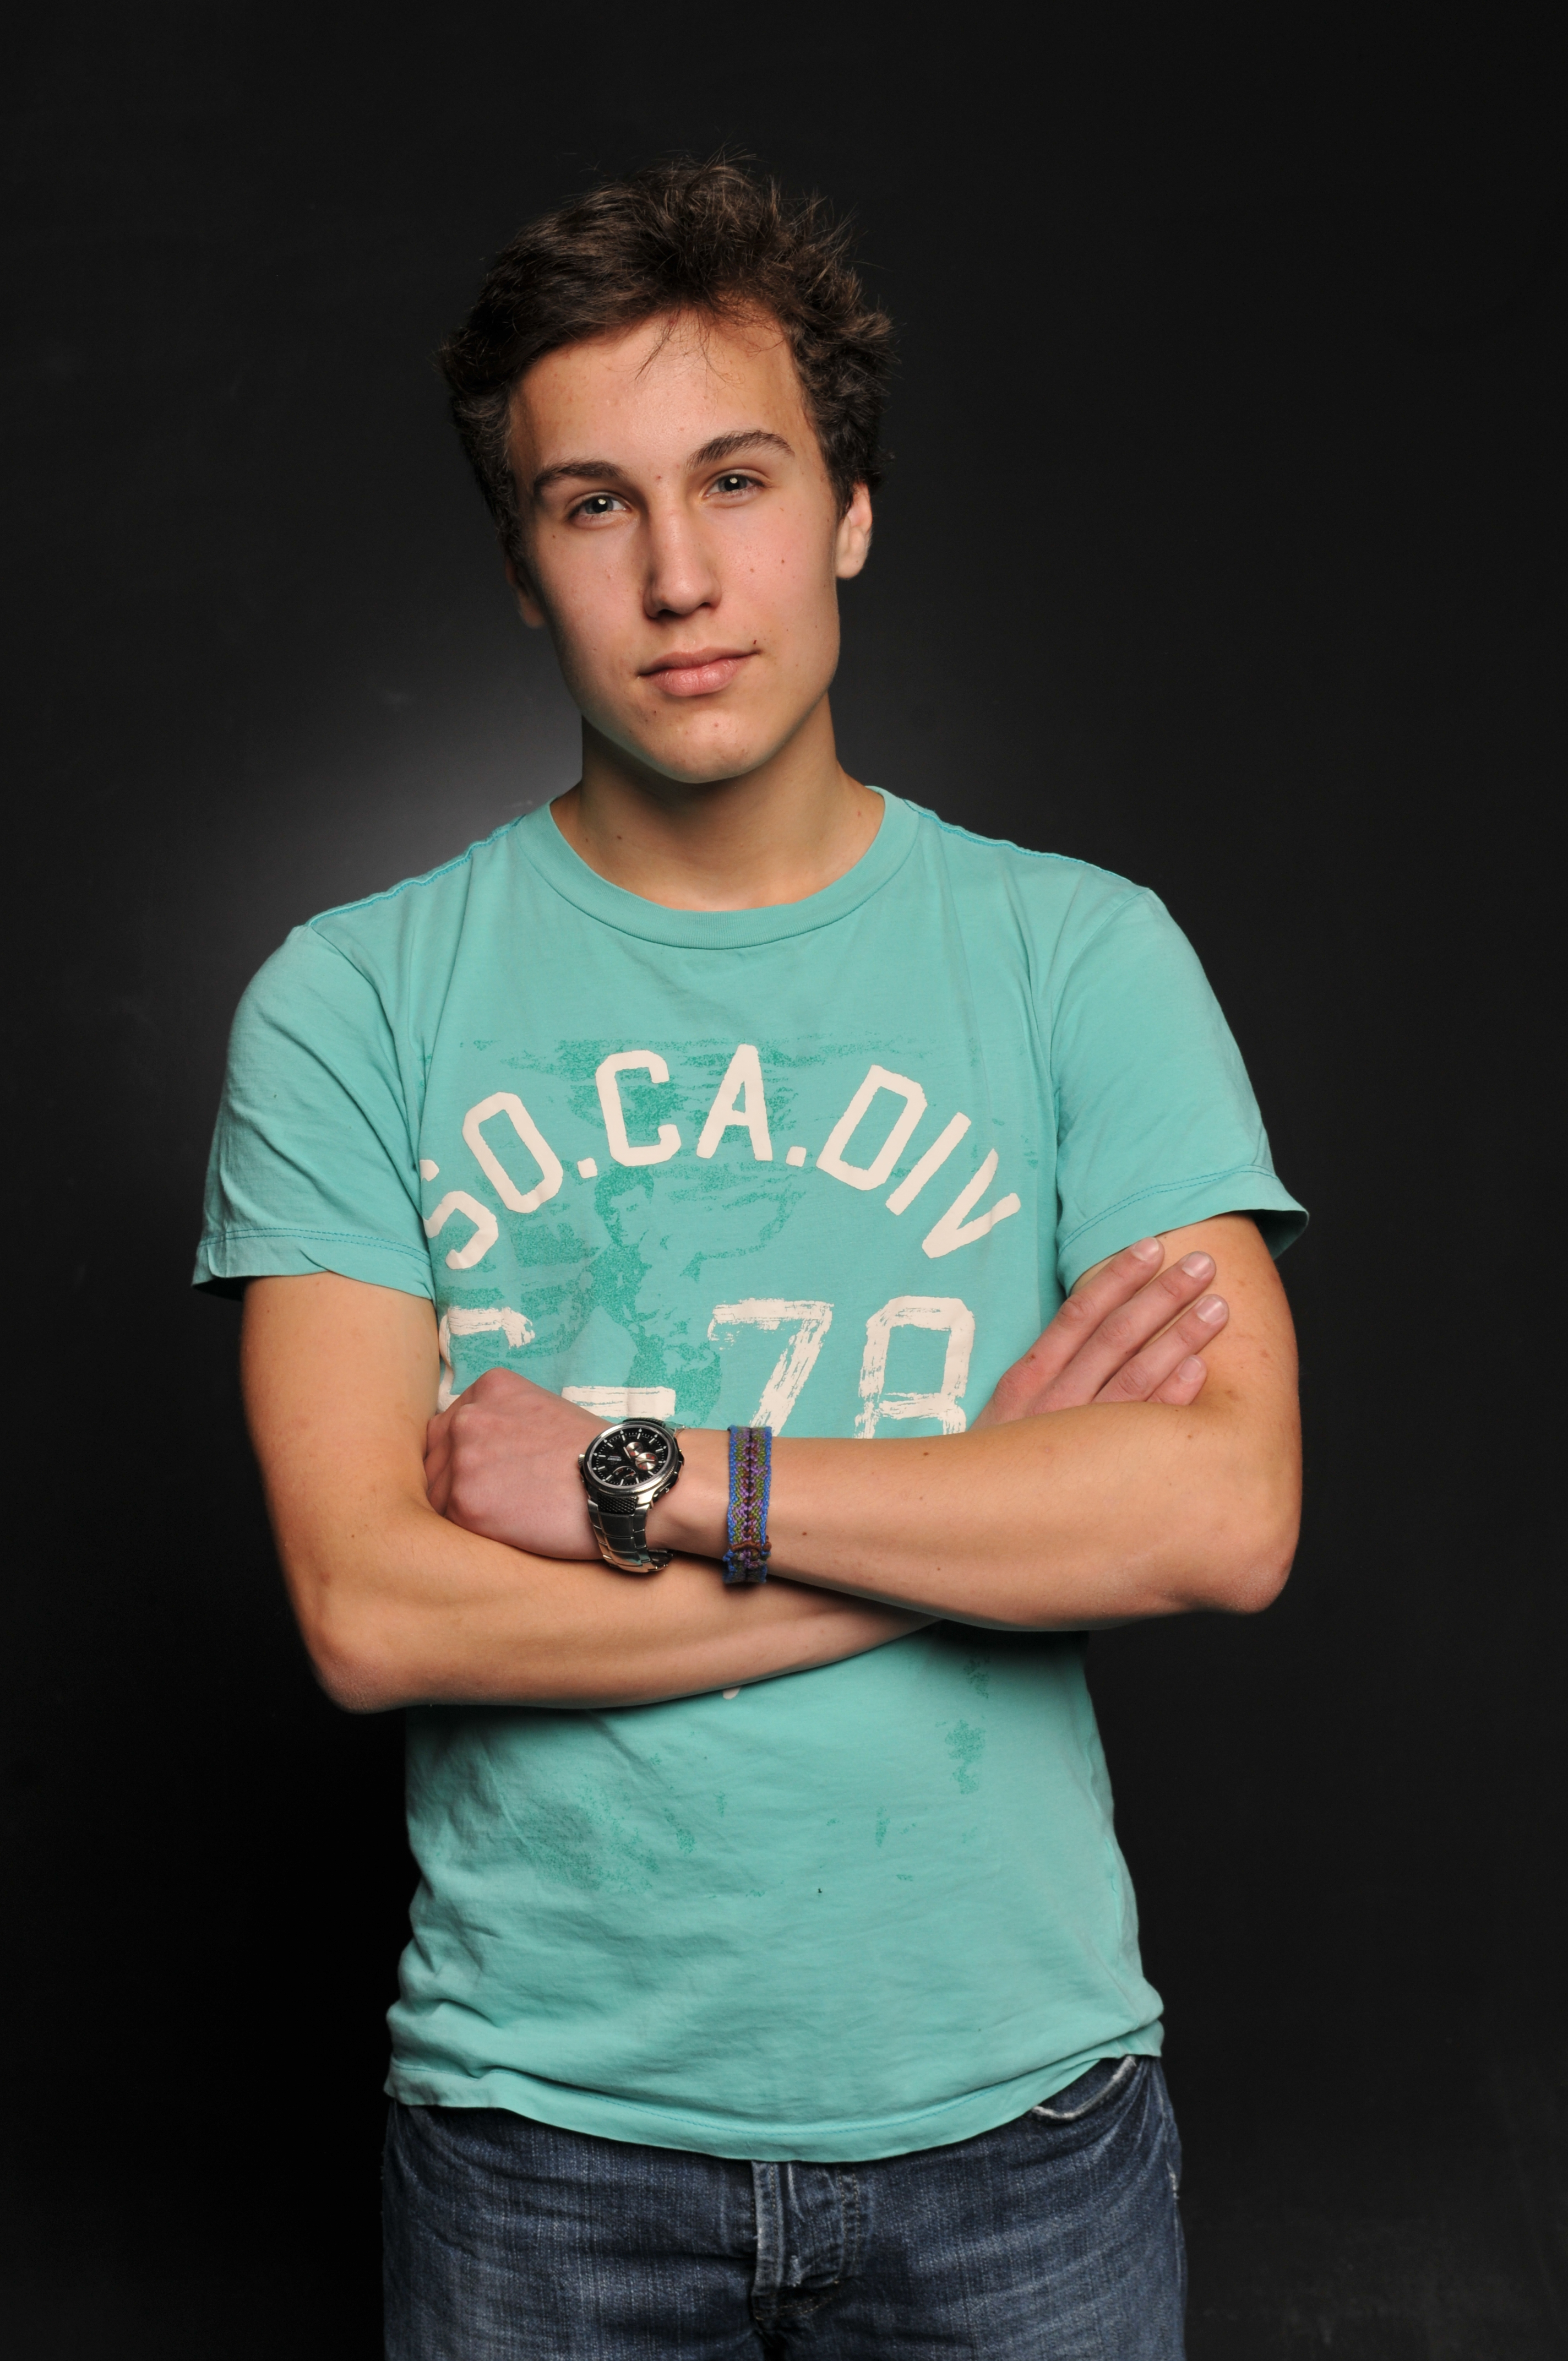
\includegraphics[scale=0.18]{days/27.03.15/images/03}}
			\caption{Stopper}
		\end{minipage}
	\end{figure}
	
	\item We installed protection from small balls and the stick in front of forward wheels.
	
	\item We made 2 framework programs for autonomus period (from the ramp and from the parking zone). To make code easier, we left only tank rotations (eg. left forward, right backward). It became possible because with optimized wheel base robot rotates more accurately.
	
	\item When we started testing automomus period, we noticed that Andymark motors' encoders didn't work. We realised, that they had been connected in a wrong way. We reconnected encoders right, but, unfortunately, it was time to go out from the competition area, so we didn't manage to make autonomus programs today.
	
\end{enumerate}
\fillpage
